% Options for packages loaded elsewhere
\PassOptionsToPackage{unicode}{hyperref}
\PassOptionsToPackage{hyphens}{url}
\PassOptionsToPackage{dvipsnames,svgnames,x11names}{xcolor}
%
\documentclass[
  letterpaper,
  DIV=11,
  numbers=noendperiod]{scrreprt}

\usepackage{amsmath,amssymb}
\usepackage{iftex}
\ifPDFTeX
  \usepackage[T1]{fontenc}
  \usepackage[utf8]{inputenc}
  \usepackage{textcomp} % provide euro and other symbols
\else % if luatex or xetex
  \usepackage{unicode-math}
  \defaultfontfeatures{Scale=MatchLowercase}
  \defaultfontfeatures[\rmfamily]{Ligatures=TeX,Scale=1}
\fi
\usepackage{lmodern}
\ifPDFTeX\else  
    % xetex/luatex font selection
\fi
% Use upquote if available, for straight quotes in verbatim environments
\IfFileExists{upquote.sty}{\usepackage{upquote}}{}
\IfFileExists{microtype.sty}{% use microtype if available
  \usepackage[]{microtype}
  \UseMicrotypeSet[protrusion]{basicmath} % disable protrusion for tt fonts
}{}
\makeatletter
\@ifundefined{KOMAClassName}{% if non-KOMA class
  \IfFileExists{parskip.sty}{%
    \usepackage{parskip}
  }{% else
    \setlength{\parindent}{0pt}
    \setlength{\parskip}{6pt plus 2pt minus 1pt}}
}{% if KOMA class
  \KOMAoptions{parskip=half}}
\makeatother
\usepackage{xcolor}
\setlength{\emergencystretch}{3em} % prevent overfull lines
\setcounter{secnumdepth}{-\maxdimen} % remove section numbering
% Make \paragraph and \subparagraph free-standing
\makeatletter
\ifx\paragraph\undefined\else
  \let\oldparagraph\paragraph
  \renewcommand{\paragraph}{
    \@ifstar
      \xxxParagraphStar
      \xxxParagraphNoStar
  }
  \newcommand{\xxxParagraphStar}[1]{\oldparagraph*{#1}\mbox{}}
  \newcommand{\xxxParagraphNoStar}[1]{\oldparagraph{#1}\mbox{}}
\fi
\ifx\subparagraph\undefined\else
  \let\oldsubparagraph\subparagraph
  \renewcommand{\subparagraph}{
    \@ifstar
      \xxxSubParagraphStar
      \xxxSubParagraphNoStar
  }
  \newcommand{\xxxSubParagraphStar}[1]{\oldsubparagraph*{#1}\mbox{}}
  \newcommand{\xxxSubParagraphNoStar}[1]{\oldsubparagraph{#1}\mbox{}}
\fi
\makeatother

\usepackage{color}
\usepackage{fancyvrb}
\newcommand{\VerbBar}{|}
\newcommand{\VERB}{\Verb[commandchars=\\\{\}]}
\DefineVerbatimEnvironment{Highlighting}{Verbatim}{commandchars=\\\{\}}
% Add ',fontsize=\small' for more characters per line
\usepackage{framed}
\definecolor{shadecolor}{RGB}{241,243,245}
\newenvironment{Shaded}{\begin{snugshade}}{\end{snugshade}}
\newcommand{\AlertTok}[1]{\textcolor[rgb]{0.68,0.00,0.00}{#1}}
\newcommand{\AnnotationTok}[1]{\textcolor[rgb]{0.37,0.37,0.37}{#1}}
\newcommand{\AttributeTok}[1]{\textcolor[rgb]{0.40,0.45,0.13}{#1}}
\newcommand{\BaseNTok}[1]{\textcolor[rgb]{0.68,0.00,0.00}{#1}}
\newcommand{\BuiltInTok}[1]{\textcolor[rgb]{0.00,0.23,0.31}{#1}}
\newcommand{\CharTok}[1]{\textcolor[rgb]{0.13,0.47,0.30}{#1}}
\newcommand{\CommentTok}[1]{\textcolor[rgb]{0.37,0.37,0.37}{#1}}
\newcommand{\CommentVarTok}[1]{\textcolor[rgb]{0.37,0.37,0.37}{\textit{#1}}}
\newcommand{\ConstantTok}[1]{\textcolor[rgb]{0.56,0.35,0.01}{#1}}
\newcommand{\ControlFlowTok}[1]{\textcolor[rgb]{0.00,0.23,0.31}{\textbf{#1}}}
\newcommand{\DataTypeTok}[1]{\textcolor[rgb]{0.68,0.00,0.00}{#1}}
\newcommand{\DecValTok}[1]{\textcolor[rgb]{0.68,0.00,0.00}{#1}}
\newcommand{\DocumentationTok}[1]{\textcolor[rgb]{0.37,0.37,0.37}{\textit{#1}}}
\newcommand{\ErrorTok}[1]{\textcolor[rgb]{0.68,0.00,0.00}{#1}}
\newcommand{\ExtensionTok}[1]{\textcolor[rgb]{0.00,0.23,0.31}{#1}}
\newcommand{\FloatTok}[1]{\textcolor[rgb]{0.68,0.00,0.00}{#1}}
\newcommand{\FunctionTok}[1]{\textcolor[rgb]{0.28,0.35,0.67}{#1}}
\newcommand{\ImportTok}[1]{\textcolor[rgb]{0.00,0.46,0.62}{#1}}
\newcommand{\InformationTok}[1]{\textcolor[rgb]{0.37,0.37,0.37}{#1}}
\newcommand{\KeywordTok}[1]{\textcolor[rgb]{0.00,0.23,0.31}{\textbf{#1}}}
\newcommand{\NormalTok}[1]{\textcolor[rgb]{0.00,0.23,0.31}{#1}}
\newcommand{\OperatorTok}[1]{\textcolor[rgb]{0.37,0.37,0.37}{#1}}
\newcommand{\OtherTok}[1]{\textcolor[rgb]{0.00,0.23,0.31}{#1}}
\newcommand{\PreprocessorTok}[1]{\textcolor[rgb]{0.68,0.00,0.00}{#1}}
\newcommand{\RegionMarkerTok}[1]{\textcolor[rgb]{0.00,0.23,0.31}{#1}}
\newcommand{\SpecialCharTok}[1]{\textcolor[rgb]{0.37,0.37,0.37}{#1}}
\newcommand{\SpecialStringTok}[1]{\textcolor[rgb]{0.13,0.47,0.30}{#1}}
\newcommand{\StringTok}[1]{\textcolor[rgb]{0.13,0.47,0.30}{#1}}
\newcommand{\VariableTok}[1]{\textcolor[rgb]{0.07,0.07,0.07}{#1}}
\newcommand{\VerbatimStringTok}[1]{\textcolor[rgb]{0.13,0.47,0.30}{#1}}
\newcommand{\WarningTok}[1]{\textcolor[rgb]{0.37,0.37,0.37}{\textit{#1}}}

\providecommand{\tightlist}{%
  \setlength{\itemsep}{0pt}\setlength{\parskip}{0pt}}\usepackage{longtable,booktabs,array}
\usepackage{calc} % for calculating minipage widths
% Correct order of tables after \paragraph or \subparagraph
\usepackage{etoolbox}
\makeatletter
\patchcmd\longtable{\par}{\if@noskipsec\mbox{}\fi\par}{}{}
\makeatother
% Allow footnotes in longtable head/foot
\IfFileExists{footnotehyper.sty}{\usepackage{footnotehyper}}{\usepackage{footnote}}
\makesavenoteenv{longtable}
\usepackage{graphicx}
\makeatletter
\newsavebox\pandoc@box
\newcommand*\pandocbounded[1]{% scales image to fit in text height/width
  \sbox\pandoc@box{#1}%
  \Gscale@div\@tempa{\textheight}{\dimexpr\ht\pandoc@box+\dp\pandoc@box\relax}%
  \Gscale@div\@tempb{\linewidth}{\wd\pandoc@box}%
  \ifdim\@tempb\p@<\@tempa\p@\let\@tempa\@tempb\fi% select the smaller of both
  \ifdim\@tempa\p@<\p@\scalebox{\@tempa}{\usebox\pandoc@box}%
  \else\usebox{\pandoc@box}%
  \fi%
}
% Set default figure placement to htbp
\def\fps@figure{htbp}
\makeatother

\KOMAoption{captions}{tableheading}
\makeatletter
\@ifpackageloaded{tcolorbox}{}{\usepackage[skins,breakable]{tcolorbox}}
\@ifpackageloaded{fontawesome5}{}{\usepackage{fontawesome5}}
\definecolor{quarto-callout-color}{HTML}{909090}
\definecolor{quarto-callout-note-color}{HTML}{0758E5}
\definecolor{quarto-callout-important-color}{HTML}{CC1914}
\definecolor{quarto-callout-warning-color}{HTML}{EB9113}
\definecolor{quarto-callout-tip-color}{HTML}{00A047}
\definecolor{quarto-callout-caution-color}{HTML}{FC5300}
\definecolor{quarto-callout-color-frame}{HTML}{acacac}
\definecolor{quarto-callout-note-color-frame}{HTML}{4582ec}
\definecolor{quarto-callout-important-color-frame}{HTML}{d9534f}
\definecolor{quarto-callout-warning-color-frame}{HTML}{f0ad4e}
\definecolor{quarto-callout-tip-color-frame}{HTML}{02b875}
\definecolor{quarto-callout-caution-color-frame}{HTML}{fd7e14}
\makeatother
\makeatletter
\@ifpackageloaded{caption}{}{\usepackage{caption}}
\AtBeginDocument{%
\ifdefined\contentsname
  \renewcommand*\contentsname{Tabla de contenidos}
\else
  \newcommand\contentsname{Tabla de contenidos}
\fi
\ifdefined\listfigurename
  \renewcommand*\listfigurename{Listado de Figuras}
\else
  \newcommand\listfigurename{Listado de Figuras}
\fi
\ifdefined\listtablename
  \renewcommand*\listtablename{Listado de Tablas}
\else
  \newcommand\listtablename{Listado de Tablas}
\fi
\ifdefined\figurename
  \renewcommand*\figurename{Figura}
\else
  \newcommand\figurename{Figura}
\fi
\ifdefined\tablename
  \renewcommand*\tablename{Tabla}
\else
  \newcommand\tablename{Tabla}
\fi
}
\@ifpackageloaded{float}{}{\usepackage{float}}
\floatstyle{ruled}
\@ifundefined{c@chapter}{\newfloat{codelisting}{h}{lop}}{\newfloat{codelisting}{h}{lop}[chapter]}
\floatname{codelisting}{Listado}
\newcommand*\listoflistings{\listof{codelisting}{Listado de Listados}}
\usepackage{amsthm}
\theoremstyle{definition}
\newtheorem{definition}{Definición}[section]
\theoremstyle{plain}
\newtheorem{theorem}{Teorema}[section]
\theoremstyle{remark}
\AtBeginDocument{\renewcommand*{\proofname}{Prueba}}
\newtheorem*{remark}{Observación}
\newtheorem*{solution}{Solución}
\newtheorem{refremark}{Observación}[section]
\newtheorem{refsolution}{Solución}[section]
\makeatother
\makeatletter
\makeatother
\makeatletter
\@ifpackageloaded{caption}{}{\usepackage{caption}}
\@ifpackageloaded{subcaption}{}{\usepackage{subcaption}}
\makeatother

\ifLuaTeX
\usepackage[bidi=basic]{babel}
\else
\usepackage[bidi=default]{babel}
\fi
\babelprovide[main,import]{spanish}
% get rid of language-specific shorthands (see #6817):
\let\LanguageShortHands\languageshorthands
\def\languageshorthands#1{}
\usepackage{bookmark}

\IfFileExists{xurl.sty}{\usepackage{xurl}}{} % add URL line breaks if available
\urlstyle{same} % disable monospaced font for URLs
\hypersetup{
  pdflang={es},
  colorlinks=true,
  linkcolor={blue},
  filecolor={Maroon},
  citecolor={Blue},
  urlcolor={Blue},
  pdfcreator={LaTeX via pandoc}}


\author{}
\date{}

\begin{document}


\chapter{Regresión por menor ángulo
(LARS)}\label{regresiuxf3n-por-menor-uxe1ngulo-lars}

\section{Intuición detrás de LARS}\label{intuiciuxf3n-detruxe1s-de-lars}

Notemos que la regresión por pasos tiene la ventaja de que llega a una
solución en a lo más \(\min\{n,p\}\) pasos, pero como mencionamos antes,
como añadimos ``mucho'' de un predictor en cada iteración, podemos, sin
darnos cuenta, eliminar alguno que fuera relevante. El algoritmo
regresión por etapas intenta resolver este problema, pero al costo de
introducir muchas iteraciones. El objetivo de el algoritmo de regresión
por menor ángulo es obtener los beneficios de ambos realizando
decisiones ``inteligente'' de que predictores añadimos en cada paso y
``cuanto'' añadimos de cada uno.

Al igual que en los dos algoritmos anteriores, la idea es añadir
predictores hasta que estemos satisfechos. Tomemos primero el caso donde

\[
X=\begin{bmatrix}
x_{1,1}&x_{1,2}\\
x_{2,1}&x_{2,2}
\end{bmatrix}.
\]

Supongamos que \(|\langle x_1,y\rangle|>|\langle x_2,y\rangle|\), de
manera que si \(\theta_1\) es el ángulo entre \(x_1, y\) y \(\theta_2\)
es el ángulo entre \(x_2,y\), entonces

\[
|\cos(\theta_1)|~||y||=|\langle x_1,y\rangle|>|\langle x_2,y\rangle|=|\cos(\theta_2)|~||y||\Rightarrow |\cos(\theta_1)|>|\cos(\theta_2)|.
\]

Esto nos dice que \(|\cos(\theta_1)|\) está más cercano a 1, y por
tanto, como \(\cos(0)=\cos(\pi)=1\), se tiene que si consideramos la
recta marcada por \(y\), entonces el ángulo formado por \(x_1\) y dicha
recta es más pequeño que el formado por \(x_2\), como se observa en la
Figura~\ref{fig-LARS}, de modo que damos un paso en esta dirección
(considerando el signo que tiene \(\langle x_1,y\rangle\)). Ahora bien,
vamos a dar un tamaño de paso muy especial. Como el algoritmo termina en
el siguiente paso y queremos llegar a la solución usual de mínimos
cuadrados, consideramos un tamaño de paso \(\hat\gamma_1\) de manera que
si \(\hat y\) es dicho estimador, entonces \(\hat y-\hat\gamma_1 x_1\)
biseque el ángulo entre \(x_1\) y \(x_2\), esto es que
\(\hat y-\hat\gamma_1 x_1\) tenga la misma correlación con \(x_1\) y
\(x_2\), de manera que nuestra estimación actual es
\(\hat\gamma_1 x_1\). Después, continuamos en la dirección marcada por
dicha bisectriz, específicamente, si \(u_2\) es el vector unitario que
biseca dicho ángulo, entonces nuestra siguiente estimación es
\(\hat\gamma_1 x_1+\hat\gamma_2 u_2\), donde \(\hat\gamma_2\) es elegido
para que la estimación final sea \(\hat y\).

\begin{figure}

\centering{

\pandocbounded{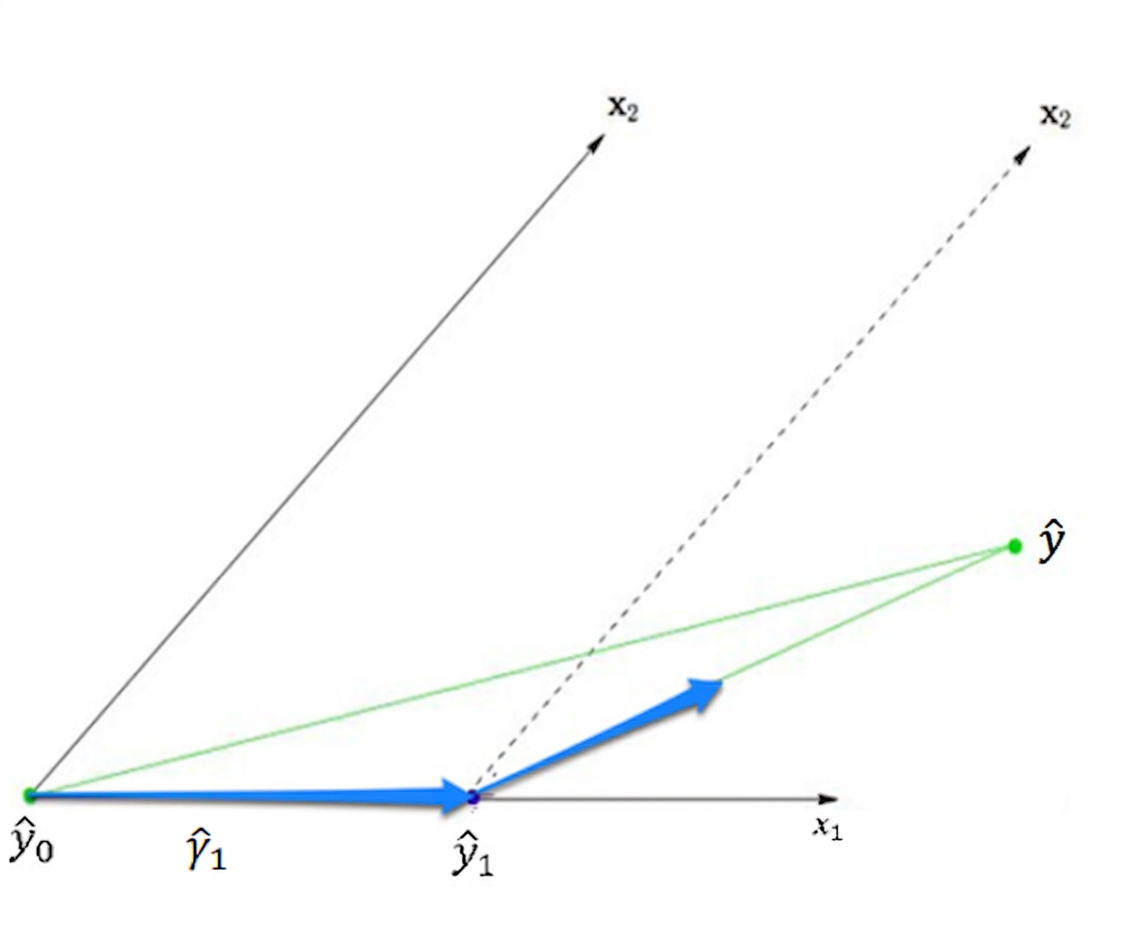
\includegraphics[keepaspectratio]{LARS.png}}

}

\caption{\label{fig-LARS}Representación gráfica de LARS en dos
dimensiones con 2 covariables.}

\end{figure}%

Notemos que el algoritmo por pasos hubiera elegido
\(\hat\gamma_1=\hat\beta_1\), mientas que el algoritmo por etapas
hubiera seguido un camino escalonado a partir de \(\hat\gamma_1 x_1\)
para llegar a \(\hat y\), mientras de que LARS elige un camino
intermedio.

\section{Algoritmo LARS en el caso
general}\label{algoritmo-lars-en-el-caso-general}

Como vimos antes, para dos vectores, el algoritmo toma la dirección de
la bisectriz entre ellos. Podemos generalizar este concepto para más
vectores:

\begin{definition}[Vector
equiangular]\protect\hypertarget{def-equia}{}\label{def-equia}

Sean \(\{x_1,\dots, x_r\}\) vectores y \(X\) la matriz cuyas columnas
son dichos vectores. Decimos que un vector \(u\) es equiangular a los
vectores \(\{x_1,\dots, x_r\}\) si

\[ X^T u=\begin{bmatrix} \alpha\\ \vdots\\ \alpha \end{bmatrix}, \]

para alguna constante \(\alpha\).

\end{definition}

Es natural preguntarse cuando podemos encontrar vectores equiangulares,
para ello tenemos el siguiente resultado:

\begin{theorem}[Existencia de vectores
equiangulares]\protect\hypertarget{thm-exis}{}\label{thm-exis}

Supongamos que \(\{x_1,\dots, x_n\}\) son linealmente independientes.
Entonces, existe un vector equiangular a dichos vectores que además es
unitario.

\end{theorem}

\begin{tcolorbox}[enhanced jigsaw, colback=white, toprule=.15mm, opacityback=0, arc=.35mm, rightrule=.15mm, breakable, leftrule=.75mm, bottomrule=.15mm, left=2mm, colframe=quarto-callout-important-color-frame]

\vspace{-3mm}\textbf{Demostración}\vspace{3mm}

Sea \(W\) la matriz con columnas \(\{x_1,\dots, x_r\}\). Notemos que
trivialmente se cumple que \(I\mathbf 1_n=\mathbf 1_n\), de manera que

\[ (W^TW)(W^TW)^{-1}\mathbf 1_n=\mathbf 1_n. \]

Así, si hacemos \(u'=W(W^TW)^{-1}\mathbf 1_n\), entonces tenemos un
múltiplo del vector \(u\) buscado. Además, como

\[ \begin{aligned} ||u'||^2&=\mathbf 1_n(W^TW)^{-1} W^TW(W^TW)^{-1}\mathbf 1_n\\ &=\mathbf 1_n(W^TW)^{-1}\mathbf 1_n \end{aligned}, \]

se tiene que

\[ u=\frac{W(W^TW)^{-1}\mathbf 1_n}{[\mathbf 1_n (W^TW)^{-1}\mathbf 1_n]^{\frac 12}}, 
\]

es un vector equiangular y además notemos que en este caso
\(\alpha=[\mathbf 1_n(W^TW)^{-1}\mathbf 1_n]^{-\frac 12}>0\).

\end{tcolorbox}

Con esto, podemos describir nuestro algoritmo. Sea
\(\hat y_{\mathcal A}\) nuestra estimación actual, donde
\(\mathcal A\subseteq \{1,\dots, \min\{n,p\}\}\) nos indica los ínidices
que los predictores que hemos agregado. Si
\(c_{\mathcal A}=X^T(y-\hat y_{\mathcal{A}})\) es el vector de
correlaciones parciales \textbf{?@eq-corrpa}, definimos

\[
\hat C_\mathcal A=\hat C=\max_j\{|c_j|\},\quad \mathcal A=\{j:|c_j|=\hat C\},
\]y también

\[
s_j=\text{sign}(c_j),\quad j\in \mathcal A.
\]

Con esto, definimos la matriz

\[ X_{\mathcal A}=(\cdots s_jx_j\cdots)_{j\in \mathcal A}, \]

donde las columnas están ordenadas de acuerdo a como van entrando
predictores. Con esto, consideremos el vector del Teorema~\ref{thm-exis}

\begin{equation}\phantomsection\label{eq-ua}{ u_\mathcal A =\frac{X_\mathcal A(X^T_{\mathcal A} X_{\mathcal A})^{-1}\mathbf 1_{|\mathcal A|}}{[\mathbf 1_{|\mathcal A|}(X_{\mathcal A}^TX_{\mathcal A})^{-1}\mathbf 1_{|\mathcal A|}]^{\frac 12}}, }\end{equation}

que es equiangular con \(\{s_jx_j\}_{j\in \mathcal A}\) y unitario.
Tenemos entonces la dirección que seguimos en nuestro siguiente paso,
resta ver la magnitud con la que aumentamos. Primeramente notemos que si
\(\gamma>0\) y definimos

\begin{equation}\phantomsection\label{eq-corrlars}{
c_j(\gamma)=x_j^T(y-\hat y_\mathcal A -\gamma u_\mathcal A)=c_j-\gamma\langle x_j,u_\mathcal A\rangle=c_j-\gamma s_jk_{\mathcal A},
}\end{equation}

donde
\(k_{\mathcal A}=[\mathbf 1_{|\mathcal A|}(X^T_{\mathcal A}X_{\mathcal A})^{-1}\mathbf 1_{|\mathcal A|}]^{-\frac 12}>0\)
. Entonces, para \(j\in \mathcal A\) se tiene que

\begin{equation}\phantomsection\label{eq-clave}{
|c_j(\gamma)|=|s_j \hat C-\gamma s_jk_{\mathcal A}|= \hat C-\gamma k_{\mathcal A},
}\end{equation}

para \(\gamma\leq \frac{\hat C}{k_\mathcal A}\). La ecuación anterior es
la clave para el algortimo funcione, esta nos dice que para valores
pequeños de \(\gamma\), \(|c_j(\gamma)|\) decrece de manera lineal para
\(j\in \mathcal A\). Además, para \(j\notin \mathcal A\), si
\(c_j\geq 0\) y \(\gamma\leq \frac{c_j}{k_\mathcal A}\), entonces

\[
|c_j(\gamma)|=c_j-\gamma k_{\mathcal A}\leq \hat C-\gamma k_{\mathcal A},
\]

y si \(c_j<0\) y \(\gamma\leq \frac{-c_j}{k_{\mathcal A}}\) , entonces

\[
|c_j(\gamma)|=-c_j-\gamma k_\mathcal A\leq \hat C-\gamma k_\mathcal A.
\]

Esto quiere decir que, partiendo de \(\gamma=0\), las correlaciones
absolutas para \(j\notin \mathcal A\) son menores que las de
\(j\in \mathcal A\) y estas últimas decrecen de manera constante. Nos
interesa entonces el valor no negativo más pequeño \(\hat \gamma\) en
tal que se cumpla la igualdad que se obtiene al igualar el lado derecho
de Ecuación~\ref{eq-clave} y Ecuación~\ref{eq-corrlars}:

\begin{equation}\phantomsection\label{eq-gamma}{
|c_j(\gamma)|=|c_j-\gamma s_j k_\mathcal A|=\hat C-\gamma k_\mathcal A,\quad j\notin \mathcal A.
}\end{equation}

En la Figura~\ref{fig-gamma} podemos ver como encontramos gráficamente
el valor de \(\hat\gamma\).

\begin{figure}

\centering{

\pandocbounded{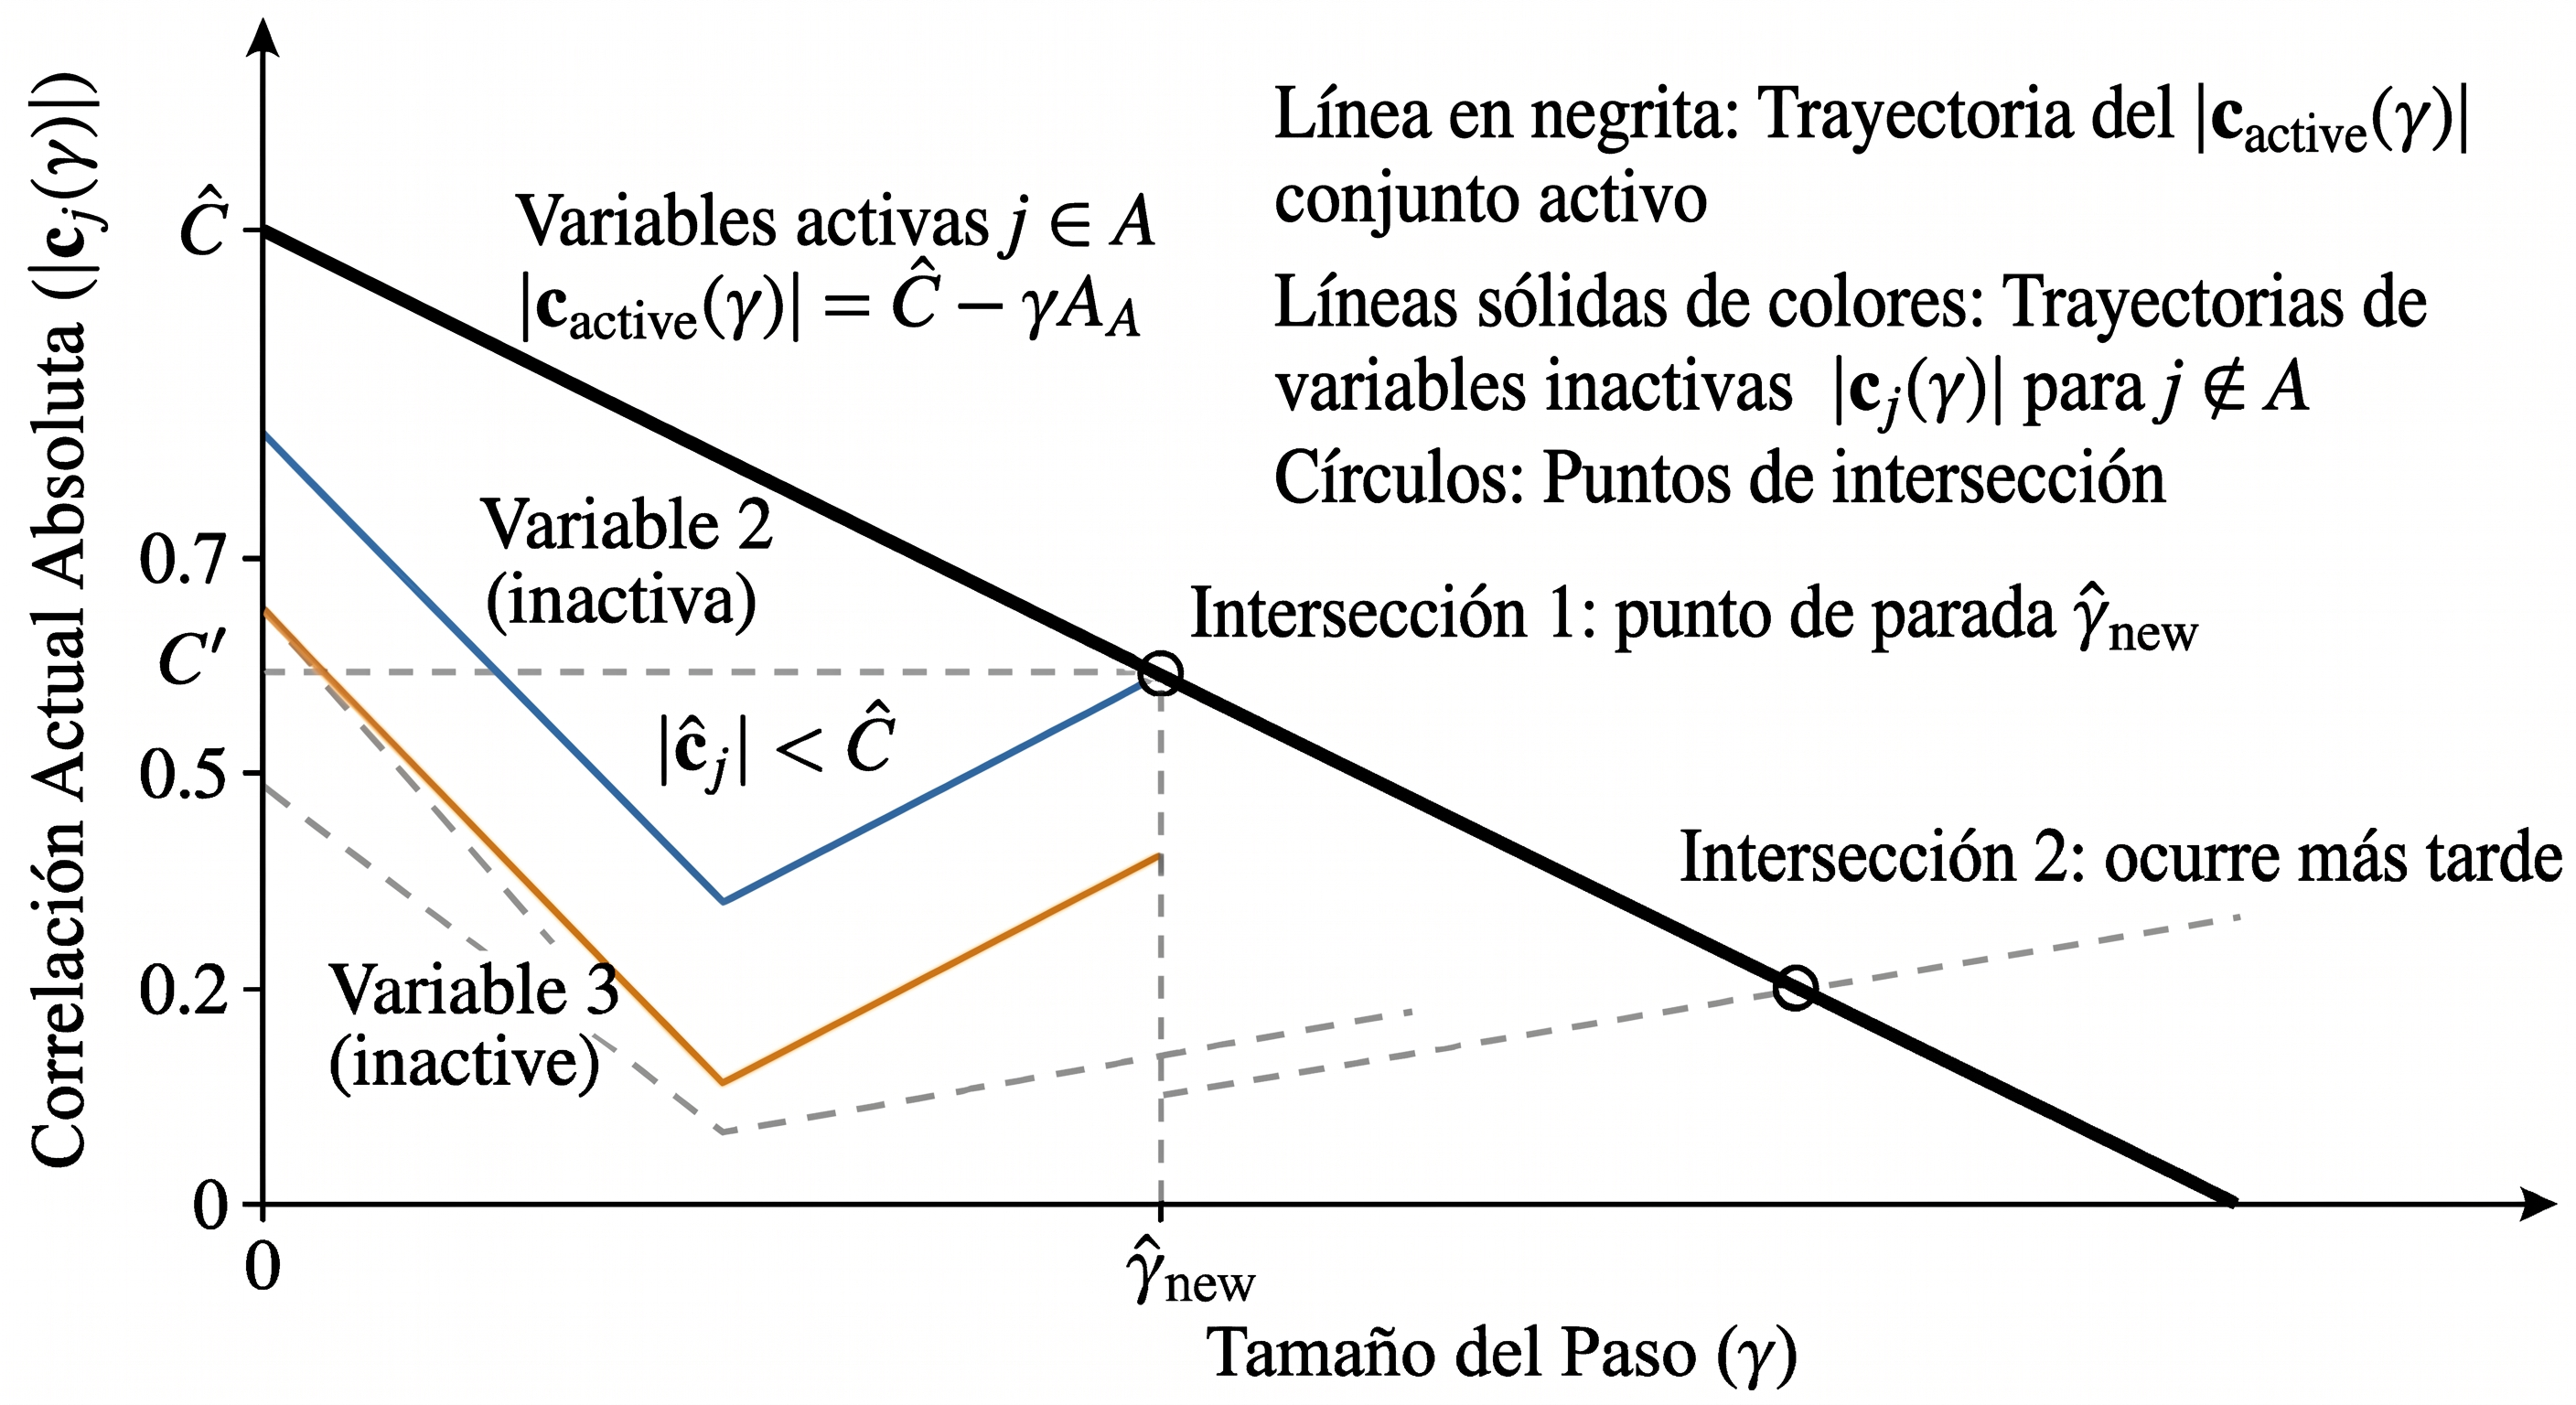
\includegraphics[keepaspectratio]{gamma.png}}

}

\caption{\label{fig-gamma}Correlaciones de las variables en A vs
correlaciones de las variables que no están en A.}

\end{figure}%

Tenemos de la Ecuación~\ref{eq-gamma} que

\begin{equation}\phantomsection\label{eq-gammareal}{
\hat\gamma=\min^+_{j\in \mathcal A^C}\left\{\frac{\hat C-c_j}{k_\mathcal A-s_jk_\mathcal A},\frac{\hat C+c_j}{k_\mathcal A+s_jk_\mathcal A}\right\}.
}\end{equation}

donde el mínimo se toma sobre valores no negativos, y notemos que se
cumple la Ecuación~\ref{eq-clave} con \(\hat\gamma\) pues si
\(c_j\geq 0\), entonces \(s_j=1\) y por tanto

\[
\hat C+c_j\leq 2 k_\mathcal A\frac{\hat C}{k_\mathcal A}\Rightarrow \frac{\hat C+c_j}{k_\mathcal A+s_jk_\mathcal A}\leq \frac{\hat C}{k_\mathcal A},
\]

y si \(c_j\leq 0\), entonces \(s_j=-1\) y por tanto

\[
\hat C-c_j\leq 2 k_\mathcal A\frac{\hat C}{k_\mathcal A}\Rightarrow \frac{\hat C-c_j}{k_\mathcal A-s_jk_\mathcal A}\leq \frac{\hat C}{k_\mathcal A}.
\]

Así, de manera compacta tenemos que nuestro algoritmo se actualiza a

\[
\mathcal A\longleftarrow \mathcal A\cup\{\hat j\},\quad \hat C\longleftarrow  \hat C-\hat\gamma k_{\mathcal A},\quad \hat y_{\mathcal A}\longleftarrow \hat y_\mathcal A+\hat\gamma u_\mathcal A,
\]donde \(\hat j\) es el \(\arg\min\) en la Ecuación~\ref{eq-gammareal}.

Lo anterior está bien definido para cada etapa del algoritmo salvo en el
último paso, pues al final \(\mathcal A^c=\varnothing\). El objetivo
final del algoritmo es recuperar la solución de mínimos cuadrados.
Supongamos que tenemos la estimación actual \(\hat y_\mathcal A\) y sea
\(\overline y_\mathcal A\) la solución de mínimos cuadrados actual.
Entonces,

\[
\overline y_\mathcal A=\hat y_\mathcal A+X_\mathcal A(X_\mathcal A^TX_\mathcal A)^{-1}X_\mathcal A^T(y-\hat y_\mathcal A)=\hat y_\mathcal A+\frac{\hat C_\mathcal A}{k_\mathcal A}u_\mathcal A,
\]pues \(\hat y_\mathcal A\) por construcción está en el espacio
generado por los vectores \(\{x_i\}_{i\in \mathcal A}\) y recordando la
Ecuación~\ref{eq-ua}. Como \(u_\mathcal A\) es unitario, se cumple que

\[
||\hat y_\mathcal A-\overline y_\mathcal A||=\frac{\hat C_\mathcal A}{k_\mathcal A},
\]entonces nunca llegamos a la solución de mínimos cuadrados, y si
queremos llegar a ella al final, requerimos que en la última iteración,

\[
\hat\gamma=\frac{\hat C_\mathcal A}{k_\mathcal A},\quad \mathcal A=\{1,\dots, \min\{n,p\}\}.
\]

Esto describe completamente a nuestro algoritmo.

\section{Con qué subconjunto nos
quedamos?}\label{con-quuxe9-subconjunto-nos-quedamos}

Si \(n<p\) nuestro algoritmo se detiene cuando ha añadido \(n\)
variables. Sin embargo, cuando \(p\geq n\) nuestro lagoritmo no se
detiene hasta añadir todas las variables. Veamos ahora un criterio que
nos ayuda a elegir un subconjunto apropiado de variables para nuestro
modelos.

\begin{definition}[Estadístico
\(C_p\)]\protect\hypertarget{def-Cp}{}\label{def-Cp}

Para el modelo de regresión lineal usual \textbf{?@eq-modelo}, si
\(\mu=X\beta\) es el vector de medias de \(y\), definimos para un ajuste
\(\hat y\) el estadístico,

\[
C_p(\hat y)=\mathbb E\left[\frac{||\hat y-\mu||^2}{\sigma^2}\right],
\]que no es más que el valor esperado del error de predicción escalado
con la varianza.

\end{definition}

Notemos que la suma de cuadrados residuales siempre se hace más pequeña
mientras más variables agregamos a nuestro modelo, mientras que nuestro
estadístico \(C_p\) no tiene por que. Ahora bien, notemos que para
\(1\leq i\leq n\) podemos escribir

\[
(\hat y_i-\mu_i)^2=(y_i-\hat y_i)^2-(y_i-\mu_i)^2+2(\hat y_i-\mu_i)(y_i-\mu_i),
\] de manera que

\[
C_p(\hat y)=\mathbb E\left[\frac{||y-\hat y||^2}{\sigma^2}\right]-n+2\sum_{i=1}^n\frac{\text{Cov}(\hat y_i,y_i)}{\sigma^2}.
\]

Usualmente no conocemos la varianza, por lo que podemos reemplazar lo
anterior con su estimador insesgado del modelo completo. Más aún, se
puede probar que bajo ciertas condiciones se tiene que

\[
C_p(\hat y_k)=\mathbb E\left[\frac{||y-\hat y_k||^2}{\hat\sigma^2}\right]-n+2k,
\]donde \(\hat y_k\) es el estimador en el \(k\)-ésimo paso de nuestro
algoritmo, y aunque no se tenga la igualdad, esta es una buena
aproximación para el estimador. Nos interesa entonces encontrar el paso
de nuestro algoritmo donde se minimice este estadístico.

\begin{tcolorbox}[enhanced jigsaw, colback=white, toprule=.15mm, opacityback=0, arc=.35mm, rightrule=.15mm, breakable, leftrule=.75mm, bottomrule=.15mm, left=2mm, colframe=quarto-callout-note-color-frame]

\vspace{-3mm}\textbf{Ejemplo}\vspace{3mm}

Consideremos de nuevo nuestra base de datos de diabetes. Al realizar la
regresión obtenemos los siguientes caminos para \(\beta\).

\begin{Shaded}
\begin{Highlighting}[]
\FunctionTok{library}\NormalTok{(}\StringTok{"lars"}\NormalTok{)}
\end{Highlighting}
\end{Shaded}

\begin{verbatim}
Loaded lars 1.3
\end{verbatim}

\begin{Shaded}
\begin{Highlighting}[]
\FunctionTok{data}\NormalTok{(diabetes)}
\NormalTok{X }\OtherTok{=}\NormalTok{ diabetes}\SpecialCharTok{$}\NormalTok{x}
\NormalTok{y }\OtherTok{=}\NormalTok{ diabetes}\SpecialCharTok{$}\NormalTok{y}

\NormalTok{res }\OtherTok{=} \FunctionTok{lars}\NormalTok{(X, y, }\AttributeTok{type =} \StringTok{"lar"}\NormalTok{)}
\FunctionTok{plot}\NormalTok{(res, }\AttributeTok{xvar =} \StringTok{"step"}\NormalTok{)}
\end{Highlighting}
\end{Shaded}

\pandocbounded{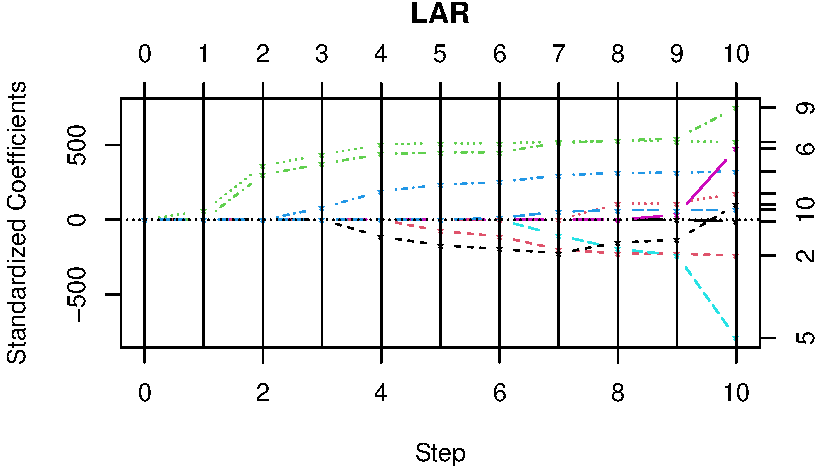
\includegraphics[keepaspectratio]{LARS_files/figure-pdf/unnamed-chunk-1-1.pdf}}

Podemos ver de nuevo que los caminos de \(\beta\) obtenidos son muy
similares a los de Lasso y regresión por etapas. Ahora bien, también
tenemos la siguiente gráfica para los estadísticos \(C_p\).

\begin{Shaded}
\begin{Highlighting}[]
\FunctionTok{plot}\NormalTok{(}\FunctionTok{seq}\NormalTok{(}\DecValTok{4}\NormalTok{,}\DecValTok{10}\NormalTok{,}\AttributeTok{by =} \DecValTok{1}\NormalTok{), res}\SpecialCharTok{$}\NormalTok{Cp[}\DecValTok{5}\SpecialCharTok{:}\DecValTok{11}\NormalTok{], }\AttributeTok{type =} \StringTok{"o"}\NormalTok{, }\AttributeTok{xlab =} \StringTok{"Step"}\NormalTok{, }\AttributeTok{ylab =} \StringTok{"Cp estimado"}\NormalTok{, }\AttributeTok{main =} \StringTok{"LAR"}\NormalTok{)}
\end{Highlighting}
\end{Shaded}

\pandocbounded{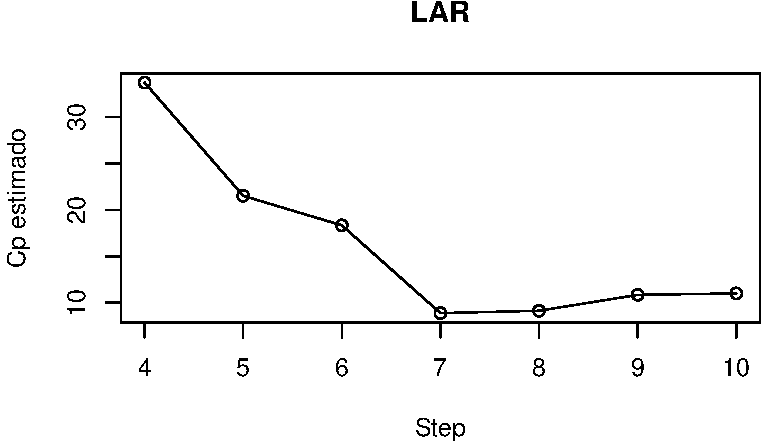
\includegraphics[keepaspectratio]{LARS_files/figure-pdf/unnamed-chunk-2-1.pdf}}

Podemos ver que el \(C_p\) estimado más pequeño fue en el paso 7 seguido
muy cerca del paso 8, por lo que ambos modelos son considerados
plausibles en este caso.

\end{tcolorbox}




\end{document}
